\documentclass[12pt,table,t]{beamer}

\usepackage{in77j}
\setbeamertemplate{bibliography item}[book]
\usebackgroundtemplate{
  
\begin{tikzpicture}
    \path [outer color = blue!5, inner color = blue!1]
      (0,0) rectangle (\paperwidth,\paperheight);
  \end{tikzpicture}}
\providecommand{\tightlist}{%
    \setlength{\itemsep}{0pt}\setlength{\parskip}{0pt}}

%\date{Primera clase\\\qquad\\24 de julio de 2014}
%\date{Pseudocódigo}

% \includeonly{tex/1.02, tex/1.03}
\includeonly{tex/1.03}

%\includeonly{tex/1.08, tex/1.08b, tex/1.08c, tex/1.08d, tex/1.08e}

% \date{Introducción al curso~~~~~Diagramas de flujo}
%\includeonly{tex/1.01, tex/1.02, tex/1.03, tex/1.04, tex/1.05, tex/1.06, tex/1.07, tex/1.07ex, tex/1.07ex2, tex/1.08, tex/1.08b, tex/1.08c, tex/1.08d, tex/1.08e}

\date{Introducción al Curso\\Conceptos de OOP}
% \includeonly{tex/2.01, tex/2.05ex, tex/2.06, tex/2.07, tex/2.08, tex/2.08ex, tex/2.09, tex/2.09b, tex/2.10, tex/2.11, tex/2.12, tex/2.16, tex/2.13}
%\includeonly{tex/2.12, tex/2.16, tex/2.13}
% \date{Introducción a Visual Basic .NET (Parte II)}
\begin{document}

%----------- titlepage ----------------------------------------------%
\begin{frame}[plain]
    \vspace{6mm}
    \centering
    \raisebox{-0.6\height}{
\includegraphics[width=70mm]{img/fcfm_dii_50a.png}}
    \raisebox{-0.5\height}{
\includegraphics[width=34mm]{img/mbe.png}}
    \vspace{6mm}
\titlepage
\end{frame}

\newcommand{\taxonomyOrg}[1][0.7]{%
  \centering\scalebox{#1}{%
    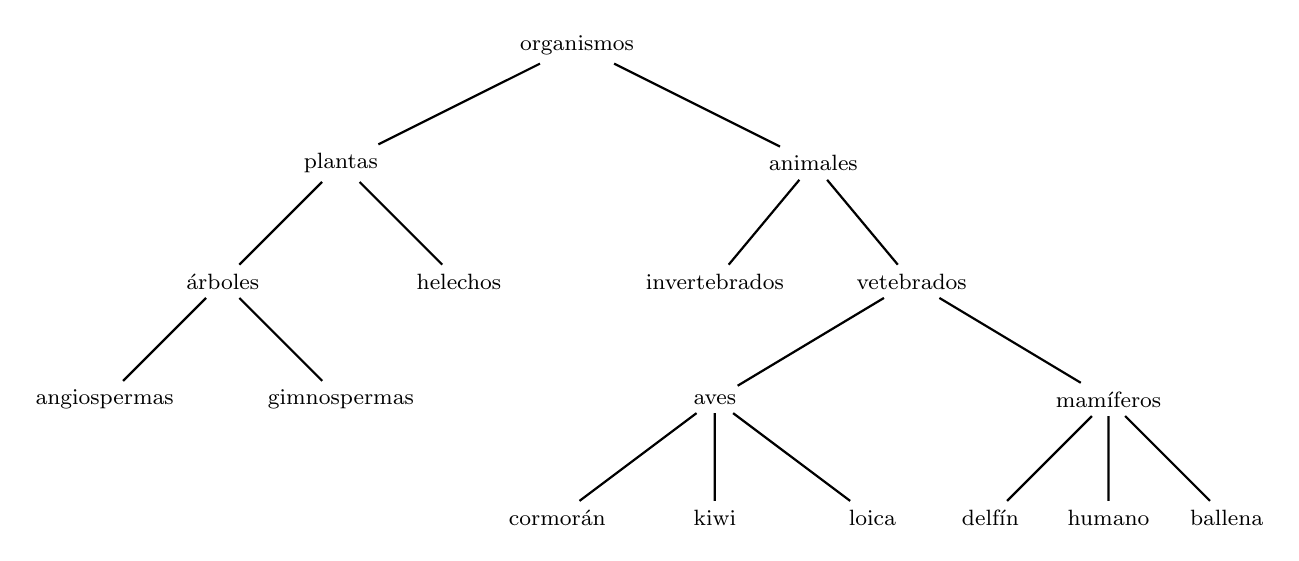
\begin{tikzpicture}
    [sibling distance=6cm,-,thick]
    \footnotesize
    \node {organismos}
      child {node {plantas}
        [sibling distance=3cm]
        child {node {árboles}
          child {node {angiospermas}}
          child {node {gimnospermas}}
        }
        child {node {helechos}}
      }
      child {node {animales}
        [sibling distance=2.5cm]
        child {node {invertebrados}}
        child {node {vetebrados}
          [sibling distance=5cm]
          child {node {aves}
            [sibling distance=2.0cm]
            child {node {cormorán}}
            child {node {kiwi}}
            child {node {loica}}
          }
          child {node {mamíferos}
            [sibling distance=1.5cm]
            child {node {delfín}}
            child {node {humano}}
            child {node {ballena}}
          }
        }
      };
    \end{tikzpicture}
  }%
}

%%%%%%%%%%%%%%%%%%%%%%%%%%

\newsavebox{\umlAgregComp}

\begin{lrbox}{\umlAgregComp}
\centering\scalebox{0.6}{%
\begin{tikzpicture}
    \umlclass[x=0,y=0]{Punto}{}{}
    \umlclass[x=-4,y=-1]{Polígono}{}{}
    \umlclass[x=4,y=-1]{Círculo}{}{}
    \umlclass[x=0,y=-4]{Estilo}{}{}
    \umlHVHcompo[anchor1=30,mult2=3..*,pos2=2.7]{Polígono}{Punto}
    \umlHVHcompo[anchor1=150,mult2=1,pos2=2.7]{Círculo}{Punto}
    \umlHVHaggreg[anchor1=-30,mult1=*,mult2=1,pos2=2.7]{Polígono}{Estilo}
    \umlHVHaggreg[anchor1=-150,mult1=*,pos1=0.3,mult2=1,pos2=2.7]{Círculo}{Estilo}
    \umlclass[x=10,y=0]{Cine}{}{}
    \umlclass[x=8,y=-3]{Película}{}{}
    \umlclass[x=12,y=-3]{Boletería}{}{}
    \umlVHVaggreg[anchor1=-110,mult1=*,mult2=*,pos1=0.3,pos2=2.8]{Cine}{Película}
    \umlVHVcompo[anchor1=-70,mult1=1,mult2=1,pos1=0.3,pos2=2.8]{Cine}{Boletería}
\end{tikzpicture}
}
\end{lrbox}

%%%%%%%%%%%%%%%%%%%%%%%%%%

\newcommand{\exAactors}{%
    \umlactor[y=-1]{Usuario}
    \umlactor[x=0,y=-5]{Cliente}
    \umlactor[x=14]{AFT}
    \umlactor[x=14,y=-4]{Banco}
    \umlactor[x=0,y=-8]{Transbank}
    \umlinherit{Cliente}{Usuario}
}

\newcommand{\exAsystem}{%
    \begin{umlsystem}[x=4]{Cajero automático}
        \umlusecase{Cargar BIP!}
        \umlusecase[y=-2]{Consulta saldo}
        \umlusecase[y=-4]{Sacar dinero}
        \umlusecase[x=2,y=-6]{Deposita sobre}
        \umlusecase[y=-8]{Recarga cajero}
        \umlusecase[x=6,y=-2,name=Valida]{Valida usuario}
        \umlinclude{usecase-1}{Valida}
        \umlinclude{usecase-2}{Valida}
        \umlinclude{usecase-3}{Valida}
    \end{umlsystem}
}
\newcommand{\exAassocs}{%
    \umlassoc{Usuario}{usecase-1}
    \umlassoc{Usuario}{usecase-2}
    \umlassoc{Usuario}{usecase-3}
    \umlassoc{Cliente}{usecase-4}
    \umlassoc{Transbank}{usecase-5}
    \umlassoc{AFT}{usecase-1}
    \umlassoc{Banco}{usecase-2}
    \umlassoc{Banco}{usecase-3}
    \umlassoc{Banco}{usecase-4}
}

\newcommand{\exUseCaseA}{%
\centering\scalebox{0.6}{%
\begin{tikzpicture}
    \exAsystem
    \exAactors
    \exAassocs
\end{tikzpicture}
}
}

\def\ucWidthB{8em}
\newcommand{\exUseCaseB}{%
\centering\scalebox{0.6}{%
\begin{tikzpicture}
    \umlactor{Cliente}
    \umlactor[y=-3]{Solicitante}
    \umlactor[y=-6]{Proveedor}
    \begin{umlsystem}[x=6]{Local comida rápida}
        \umlusecase[name=orden]{Ordenar pedido}
        \umlusecase[name=contrata,width=\ucWidthB,y=-2]{Contratar personal}
        \umlusecase[name=suministros,width=\ucWidthB,x=0,y=-4]{Pide más suministros}
        \umlusecase[name=reportes,x=3,y=-6]{Genera reportes}
        \umlusecase[name=inventario,width=\ucWidthB,x=-1,y=-8]{Control de inventario}
    \end{umlsystem}
    \umlactor[x=14,y=0]{Empleado}
    \umlactor[x=14,y=-5]{Administrador}
    \umlinherit{Administrador}{Empleado}
    \umlassoc{Cliente}{orden}
    \umlassoc{Empleado}{orden}
    \umlassoc{Solicitante}{contrata}
    \umlassoc{Administrador}{contrata}
    \umlassoc{Proveedor}{suministros}
    \umlassoc{Administrador}{suministros}
    \umlassoc{Administrador}{reportes}
    \umlinclude{suministros}{inventario}
    \umlinclude{reportes}{inventario}
\end{tikzpicture}
}
}

\newcommand{\exUseCaseDices}{%
\centering\scalebox{0.6}{%
\begin{tikzpicture}
    \umlactor{Jugador}
    \begin{umlsystem}[x=4]{Juego de dados}
        \umlusecase[name=jugar]{Jugar Dados}
    \end{umlsystem}
    \umlassoc{Jugador}{jugar}
\end{tikzpicture}
}
}

\newcommand{\exAdmProps}{%
    \umlclass[x=0,type=abstract]{Inmueble}%
      {--id : Integer\\--año : Integer\\--dirección : String}%
      {+asignaDuenno(dueño : Propietario)}%
    \umlclass[x=10]{Propietario}%
      {--nombre : String\\--rut : String}%
      {+agrInmueble(nvoInm : Inmueble)}%
    \umlclass[x=-3,y=-4.5]{Casa}%
      {--tienePatio : boolean}%
      {}%
    \umlclass[x=3,y=-4.5]{Departamento}%
      {--numPiso : Integer\\--numDepto : String}%
      {}%
    \umlVHVinherit[weight=0.45,anchor2=-120]{Casa}{Inmueble}
    \umlVHVinherit[weight=0.45,anchor2=-60]{Departamento}{Inmueble}
    \umlassoc[attr1=|*,attr2=dueño|1]{Inmueble}{Propietario}
}
\newcommand{\exAdmPropsInteraction}{%
    \exAdmProps
    \umlclass[x=-8,y=4]{AdmPropiedades}%
      {--inmId : Integer\\--inmAño : Integer\\--inmDir : String}%
      {+{datosInmueble(id,año,dir,nombre,rut)}\\+datosCasa(patio : boolean)\\+{datosDepto(np : Integer, nd : String)}\\+concretarIngreso() : boolean}
    \umlHVuniassoc[anchors=-20 and 90,attr2=inmblObj|0..1]{AdmPropiedades}{Inmueble}
    \umlHVuniassoc[anchors=0 and 90,attr2=propObj|0..1]{AdmPropiedades}{Propietario}
    \umlVHdep{AdmPropiedades}{Casa}
    \umlHVHdep[anchors=20 and 0,arm2=88mm]{AdmPropiedades}{Departamento}
}

\include{tex/1.01}
\include{tex/1.02}
\include{tex/1.03}
% \include{tex/1.03}
% \include{tex/1.04}
% \include{tex/1.05}
% \include{tex/1.06}
% \include{tex/1.07}
% \include{tex/1.07ex}
% \include{tex/1.07ex2}
% \include{tex/1.08}
% \include{tex/1.08b}
% \include{tex/1.08c}
% \include{tex/1.08d}
% \include{tex/1.08e}
% \part{1}
% \include{tex/2.01}
% \include{tex/2.06}
% \include{tex/2.05ex}
% \include{tex/2.07}
% \part{2}
% \include{tex/2.08}
% \include{tex/2.08ex}
% \include{tex/2.09}
% \include{tex/2.09b}
% \include{tex/2.10}
% \include{tex/2.11}
% \part{3}
% \include{tex/2.12}
% \include{tex/2.16}
% \include{tex/2.13}
\end{document}
